\documentclass[12pt]{article}
\usepackage[english]{babel}
\usepackage[utf8]{inputenc}

%% Pointer to 'default' preamble
% pacakages and definitions

\usepackage{geometry}
\geometry{
	letterpaper, 
	portrait, 
	top=.75in,
	left=.8in,
	right=.75in,
	bottom=.5in		} 	% Page Margins
	
%% additional packages for nice things
\usepackage{amsmath} 	% for most math
\usepackage{commath} 	% for abs
\usepackage{lastpage}	% for page count
\usepackage{amssymb} 	% for therefore
\usepackage{graphicx} 	% for image handling
\usepackage{wrapfig} 	% wrap figures
\usepackage[none]{hyphenat} % for no hyphenations
\usepackage{array} 		% for >{} column characterisctis
\usepackage{physics} 	% for easier derivative \dv....
\usepackage{tikz} 		% for graphic@!
\usepackage{circuitikz} % for circuits!
\usetikzlibrary{arrows.meta} % for loads
\usepackage[thicklines]{cancel}	% for cancels
\usepackage{xcolor}		% for color cancels
\usepackage[per-mode=fraction]{siunitx} % for si units and num
\sisetup{group-separator = {,}, group-minimum-digits = 3} % additional si unit table functionality

\usepackage{fancyhdr} 	% for header
\usepackage{comment}	% for ability to comment out large sections
\usepackage{multicol}	% for multiple columns using multicols
\usepackage[framed,numbered]{matlab-prettifier} % matlab sytle listing
\usepackage{marvosym} 	% for boltsymbol lightning
\usepackage{pdflscape} 	% for various landscape pages in portrait docs.
%\usepackage{float}
\usepackage{fancyvrb}	% for Verbatim (a tab respecting verbatim)
\usepackage{enumitem}	% for [resume] functionality of enumerate
\usepackage{spreadtab} 	% for using formulas in tables}
\usepackage{numprint}	% for number format in spread tab
\usepackage{subcaption} % for subfigures with captions
\usepackage[normalem]{ulem} % for strike through sout

% for row colors in tables....
\usepackage{color, colortbl}
\definecolor{G1}{gray}{0.9}
\definecolor{G2}{rgb}{1,0.88,1}%{gray}{0.6}
\definecolor{G3}{rgb}{0.88,1,1}

% For table formatting
\usepackage{booktabs}
\renewcommand{\arraystretch}{1.2}
\usepackage{floatrow}
\floatsetup[table]{capposition=top} % put table captions on top of tables

% Caption formating footnotesize ~ 10 pt in a 12 pt document
\usepackage[font={small}]{caption}

%% package config 
\sisetup{output-exponent-marker=\ensuremath{\mathrm{E}}} % for engineer E
\renewcommand{\CancelColor}{\color{red}}	% for color cancels
\lstset{aboveskip=2pt,belowskip=2pt} % for more compact table
%\arraycolsep=1.4pt\def
\setlength{\parindent}{0cm} % Remove indentation from paragraphs
\setlength{\columnsep}{0.5cm}
\lstset{
	style      = Matlab-editor,
	basicstyle = \ttfamily\footnotesize, % if you want to use Courier - not really used?
}
\renewcommand*{\pd}[3][]{\ensuremath{\dfrac{\partial^{#1} #2}{\partial #3}}} % for larger pd fracs
\renewcommand{\real}[1]{\mathbb{R}\left\{ #1 \right\}}	% for REAL symbol
\newcommand{\imag}[1]{\mathbb{I}\left\{ #1 \right\}}	% for IMAG symbol
\definecolor{m}{rgb}{1,0,1}	% for MATLAB matching magenta
	
%% custom macros
\newcommand\numberthis{\addtocounter{equation}{1}\tag{\theequation}} % for simple \numberthis command

\newcommand{\equal}{=} % so circuitikz can have an = in the labels
\newcolumntype{L}[1]{>{\raggedright\let\newline\\\arraybackslash\hspace{0pt}}m{#1}}
\newcolumntype{C}[1]{>{\centering\let\newline\\\arraybackslash\hspace{0pt}}m{#1}}
\newcolumntype{R}[1]{>{\raggedleft\let\newline\\\arraybackslash\hspace{0pt}}m{#1}}

%% Header
\pagestyle{fancy} % for header stuffs
\fancyhf{}
% spacing
\headheight 29 pt
\headsep 6 pt

%% Header
\rhead{Thad Haines \\ Page \thepage\ of \pageref{LastPage}}
\chead{Thoughts on how to simulate \\ bringing a generator online  }
\lhead{Research \\ 08/26/20}

\usepackage[hidelinks]{hyperref} % allow links in pdf
\usepackage{setspace}
\usepackage{multicol}
\usepackage{lscape}
%\usepackage{minted}

\begin{document}
\onehalfspacing
\paragraph{Document Purpose / Intent} \ \\
An extended term case may require the insertion of new, or additional, modeled generation resources.
There is currently no known method in PST to increase inertial generation during a simulation.
Additionally, there seemed to be minor confusion/forgetfulness as to how PST currently handles tripping a generator.
A closer look into what happens when machines are tripped off may provide some insight into a method to `un-trip', or insert, generators.


\paragraph{How generators are currently tripped in PST} \ \\
During simulation initialization, \verb|g.mac.mac_trip_flags| is initialized as a row vector of zeros that correspond to the \verb|mac_con| array, and 
\verb|g.mac.mac_trip_states| variable is set to zero. %\verb|g.mac.mac_trip_states|  ( appears unused).
To trip a generator, a \verb|mac_trip_flag| is set to $1$ via the user generated \verb|mac_trip_logic| code.
The \verb|mac_trip_logic| is executed in the \verb|initStep| function which alters \verb|g.mac.mac_trip_flags| to account for any programmed trip.
Specifically, a $0$ in the \verb|g.mac.mac_trip_flags| row vector is changed to a 1 to signify a generator has tripped.

The \verb|g.mac.mac_trip_flags| vector is summed in the \verb|networkSolution| (\verb|networkSoltuionVTS|).
If the resulting sum is larger than 0.5, the line number connected to the generator in the \verb|g.line.line_sim| is found and the reactance is set to infinity (1e7).
The reduced y matrices are then recalculated and used to solve the network solution via an \verb|i_simu| call.

If derivatives of the tripped machine are not set to zero (as the current VTS method does), the generator's speed increases, mechanical power output eventually drops to zero/near-zero, and the attached exciter Efd appears to approach 1.

%Realistically, Pmech and all P and Q limits should also probably be set to zero which may `clean up' values.
\subparagraph{Performance Note}
If a machine is tripped, altered reduced Y matrices are generated every simulation step.
This repeated action could be reduced via use of globals.
\begin{itemize}
\item create new globals handling the Y matrices selected during the network solution.
\item create an \verb|old_mac_trip_flags|
\item compare \verb|old_mac_trip_flags| to \verb|mac_trip_flags|
\item if there has been a new trip, update associated Y matrix globals
\item if there hasn't been a new trip, but a machine has tripped, use the stored Y matrix
\end{itemize} 
This is merely a calculation reduction and not required, but may result in a noticeable speed up.

\pagebreak
\paragraph{Initial 'Un-trip' Thoughts} \ \\
If the trip flag is changed from 1 to zero - the reactance would return to normal, essentially reconnecting the generator to the system.
However, the calculated states and derivatives would be no longer be synchronized and probably cause all sorts of issues/transients.

The machine model may be re-initialized via the use of the 0 flag and setting $i$ to the internal number of the generator to re-initialize.
This would require knowing what type of machine model is tripped so the proper function call is used.
% are indices of machines tracked? or just number of models?
The effects of such action is untested - a simple test case should be created and attempted.

Basically:
create small system with multiple generators, trip a generator, allow system to regain steady state, reconnect generator by setting machine trip flag back to zero.
Observe results and attempt to resolve issues.

\paragraph{`Un-trip' Method 1 - Alter Aggregate Generator } \ \\
This method includes altering a machine's base during simulation to imitate the addition/reduction of an aggregate generator.
It would require recalculation of all \verb|mac_pot| values used in model calculations.
Additionally, the monitoring of what is actually occurring may be obfuscated by the fact that any gains in capacity would be added to the existing aggregate value.
This method was not predicted as being viable due to foreseen complexity/unavoidable transients.


\paragraph{`Un-trip' Method 2 - Stand alone Generator } \ \\
Account for all generators that may, or may not, be added into the system during creation of the system data file (case).
Handle model re-initializations and bypasses as required to mimic actual procedure of connecting a generator to a synchronous system.

\paragraph{Test System}\ A simple 3 machine system was created where all machines have governors, exciters, and pss.
Parameters are essentially the same except for MVA base for each generator which was 500, 200, and 100 for generator 1, 2, and 3, respectively

\begin{center}
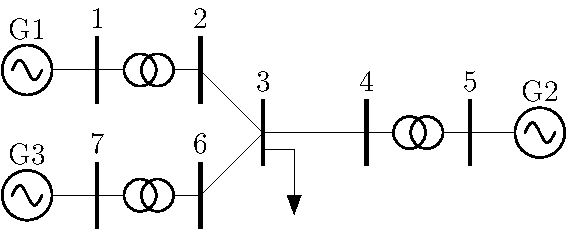
\includegraphics[width=.85\linewidth]{200831-3mach7bus}
\end{center}

\pagebreak
\begin{landscape}

\paragraph{Initial Experimental Results}
Using the previous notes as a guide, a 3 machine scenario was created where generator 3 will trip off, then attempt to be reconnected with minimal transient behavior.
Initial results are appear promising.
All transient behavior may not be eliminated, but could possibly reduced by reseting set point values and then ramping to the new desired setting (most notably the exciter reference voltage).
\begin{center}
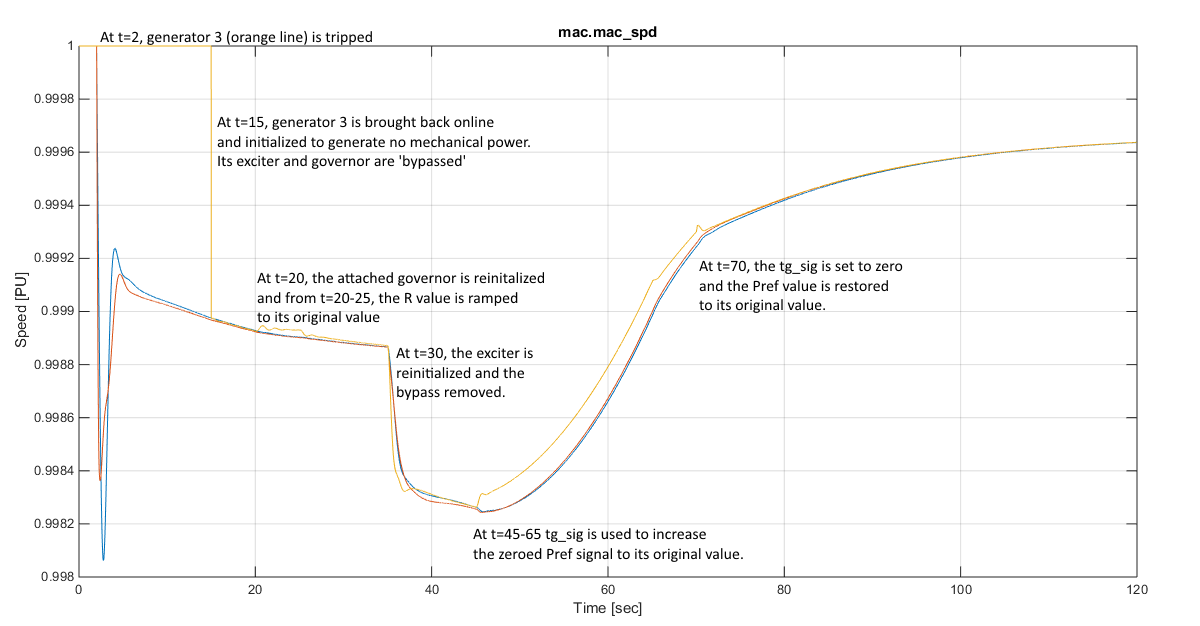
\includegraphics[width=.95\linewidth]{machineSpeedsNotes}
\end{center}

The exciter ramping up field voltage (and generating vars) caused the speed dip at t=35.
The exciter is required to be connected before mechanical power is ramped, else voltage collapse occurs and the machine `runs away'.
The machine speeds do not return to 1 as the mechanical powers do not fully restore.
The $P_{ref}$ setting of the tripped governor appears to not end at the 0.5 it is set to, or the Pref value is scaled somewhere in the model that has been missed.
\end{landscape}

\paragraph{Various Other Result Plots} \ \\
\begin{center}
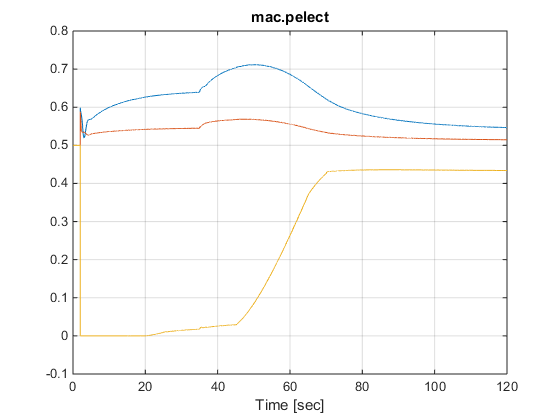
\includegraphics[width=.49\linewidth]{pelect} %
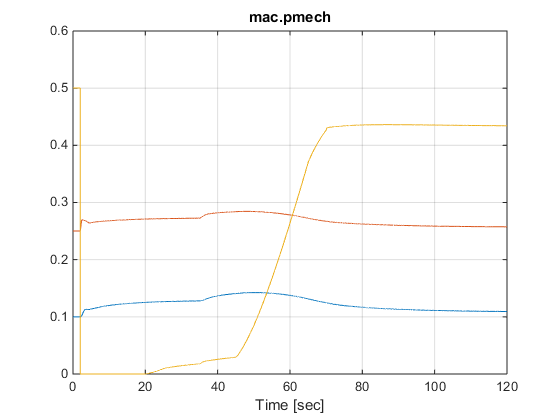
\includegraphics[width=.49\linewidth]{pmech}

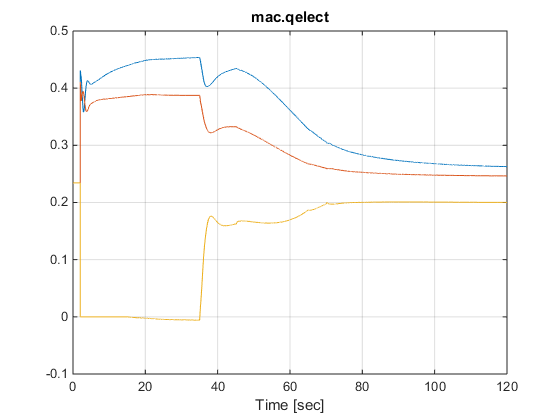
\includegraphics[width=.49\linewidth]{qelect} %
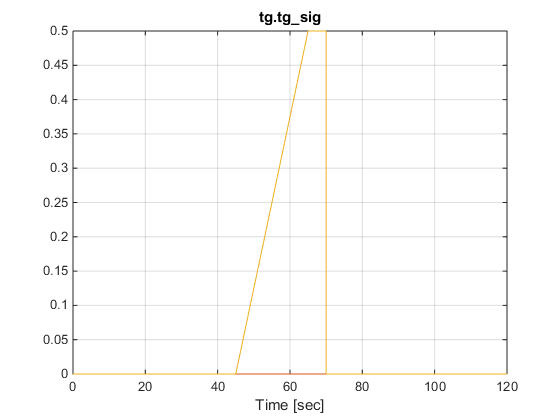
\includegraphics[width=.49\linewidth]{tg_sig}


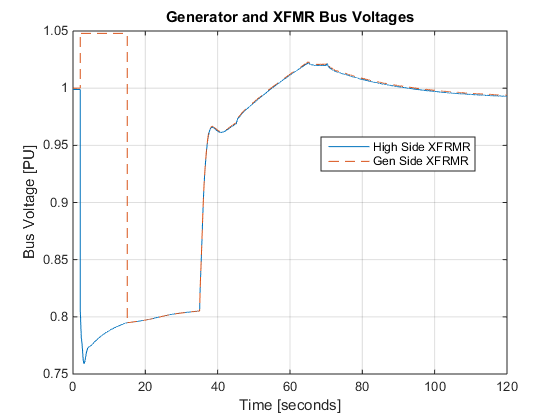
\includegraphics[width=.49\linewidth]{genBusV} %
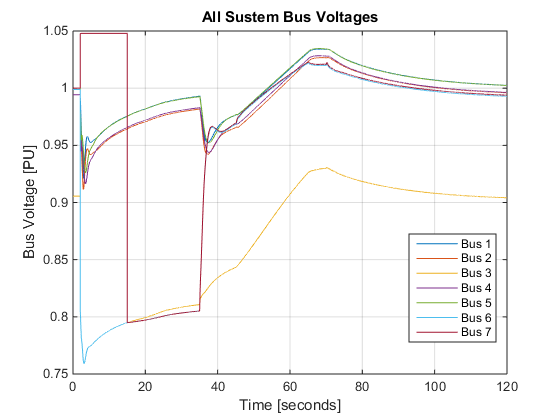
\includegraphics[width=.49\linewidth]{sysBusV} 
\end{center}

\pagebreak
\paragraph{Refined Results} \ \\
The distinct `un-trip' event time line is as follows:
\begin{itemize}
\itemsep 0 em
\item $t=0$ - System initialized
\item $t=5$ - Generator 3 trips off.
Associated derivatives, $P_{mech}$, and governor $P_{ref}$ set to zero.
\item $t=15$ - Generator 3 re-synced to system and infinite reactance reset to original value. 
Negative Q flow between buss 6-3 is observed.
\item $t=20-25$ - The governor attached to Generator 3 is reinitialized and the $R$ value is ramped to its original value. 
This causes some mechanical power to be generated by Generator 3 which also causes minor transients in system machine speed.
\item $t=35$ - Exciter is re-initialized and the bypass is removed.
This causes more reactive power flow into generator 3, the attached bus voltages to decrease, and system speed to increase slightly. 
\item $t=45-65$ - Ramping the governor $P_{ref}$ to the original value increases system speed  and real power flow from Generator 3.
\item $t=80-100$ - Ramping exciter reference voltage to original value decreases system speed and increases reactive power flow from Generator 3.
\item $t=120$ - Simulation End
\end{itemize}
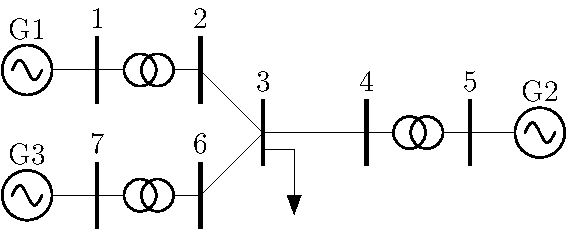
\includegraphics[width=\linewidth]{200831-3mach7bus}

%\paragraph{Observations of Note:}
%\begin{itemize}
%\item The re-connected speed of Generator 3 was set to match Generator 1.
%\item The ramping of R causes a minor 
%\item The exciter was not being initialized to the correct reference voltage time index (i.e. \verb|g.exc.exc_pot(x,3)| referenced index 1 instead of $k$ ). This has been resolved however the exciter still produces a transient when it is bypassed.
%\end{itemize}

\pagebreak
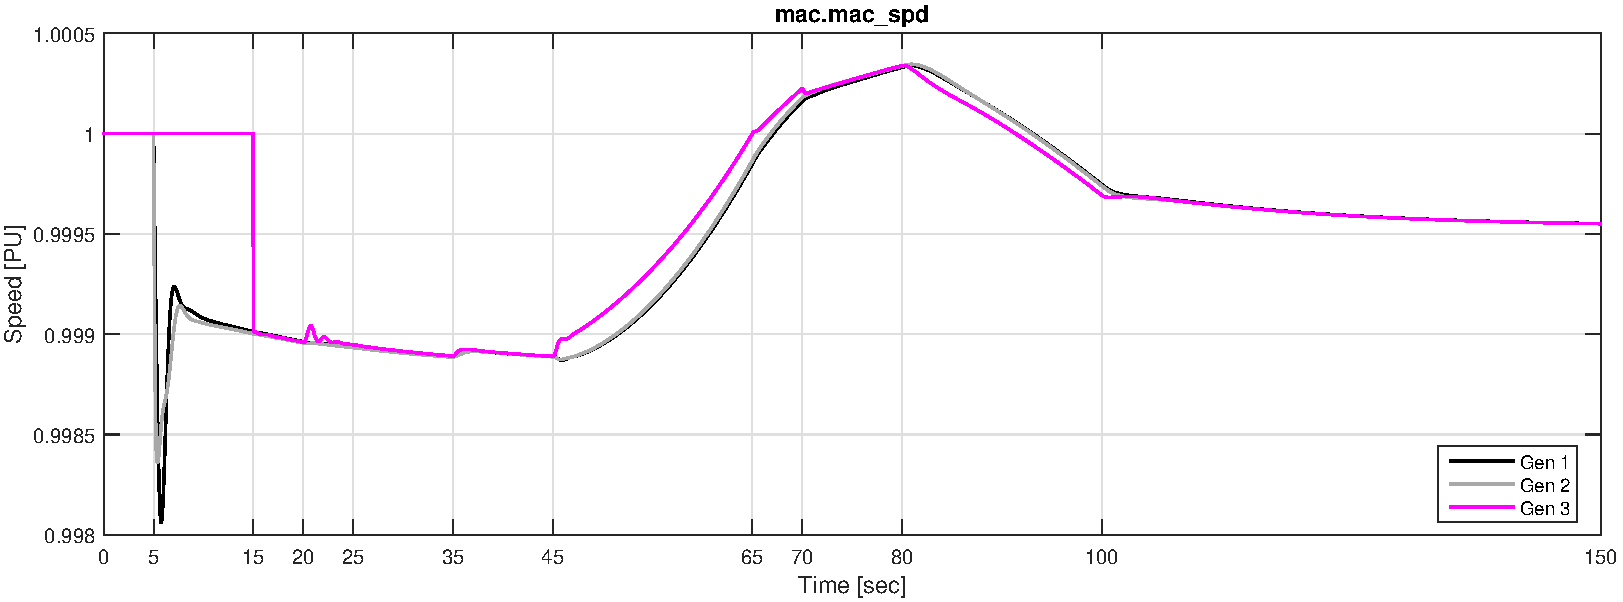
\includegraphics[width=\linewidth]{distinctSpeed}
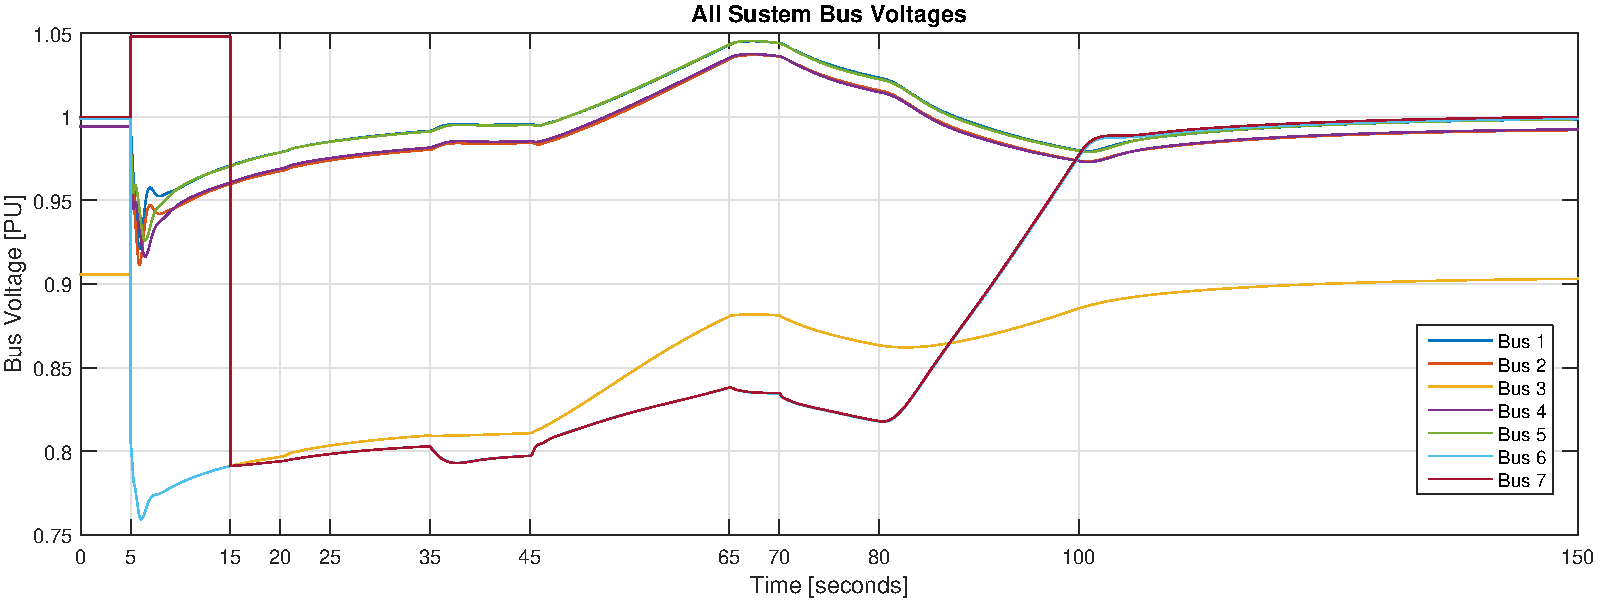
\includegraphics[width=\linewidth]{distinctBusV}


\pagebreak
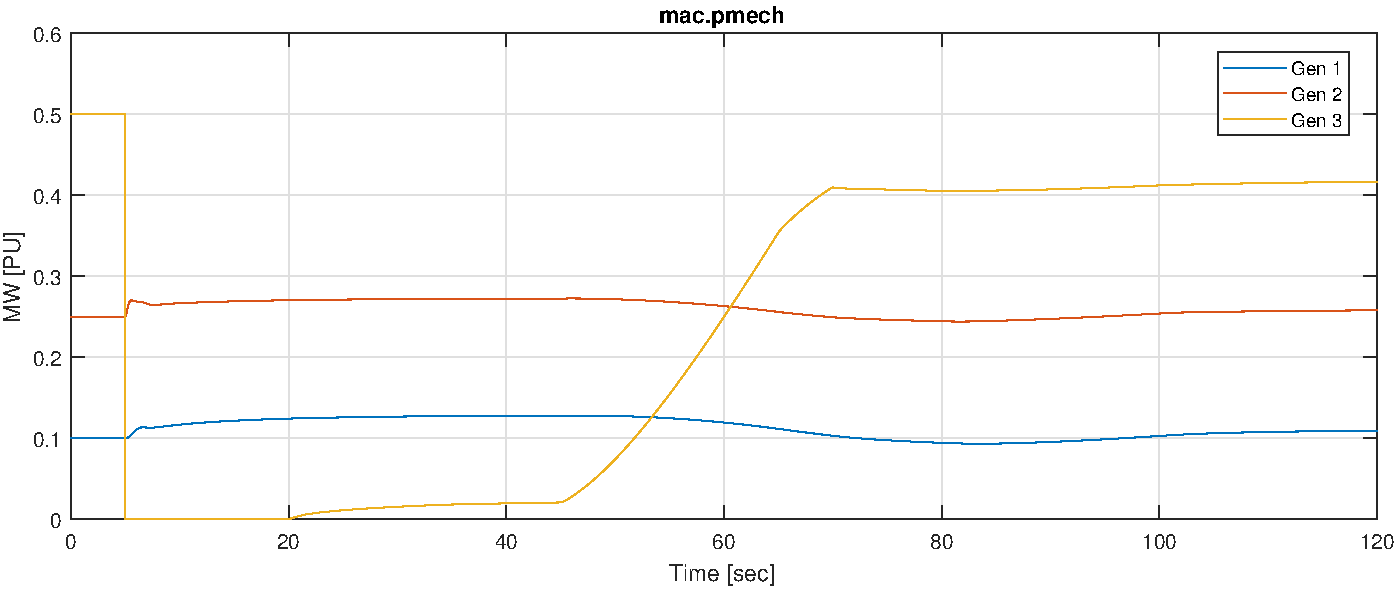
\includegraphics[width=\linewidth]{distinctPmech}
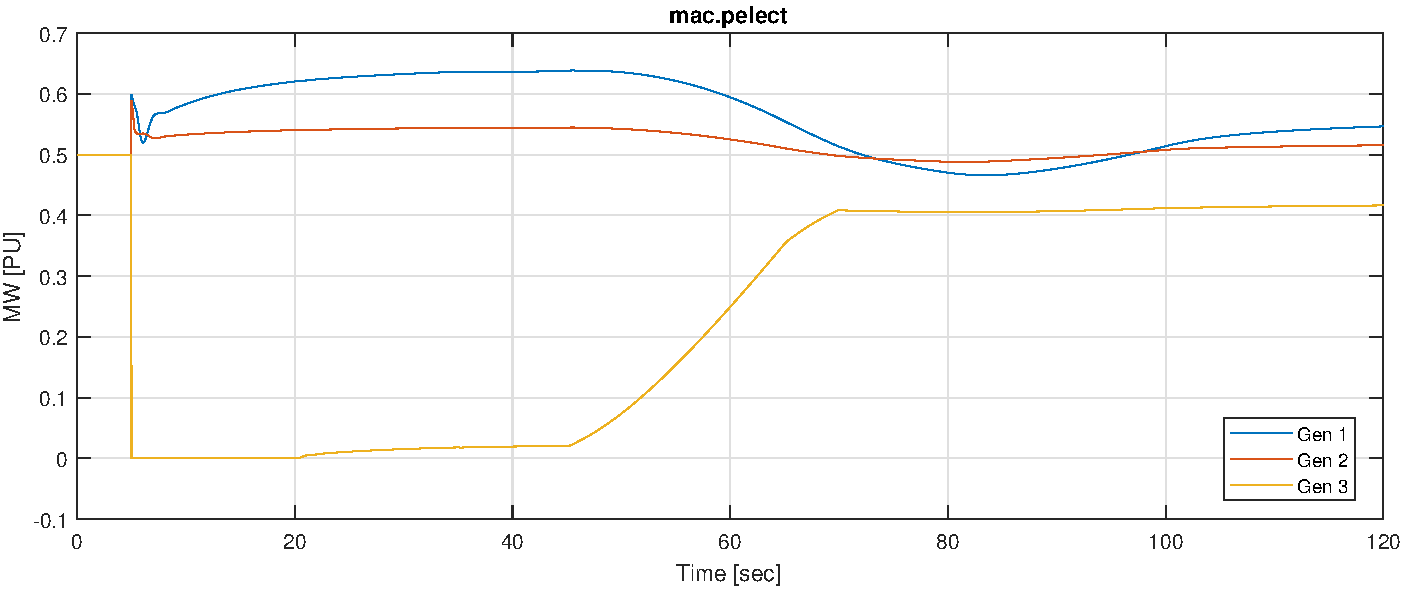
\includegraphics[width=\linewidth]{distinctPelect}
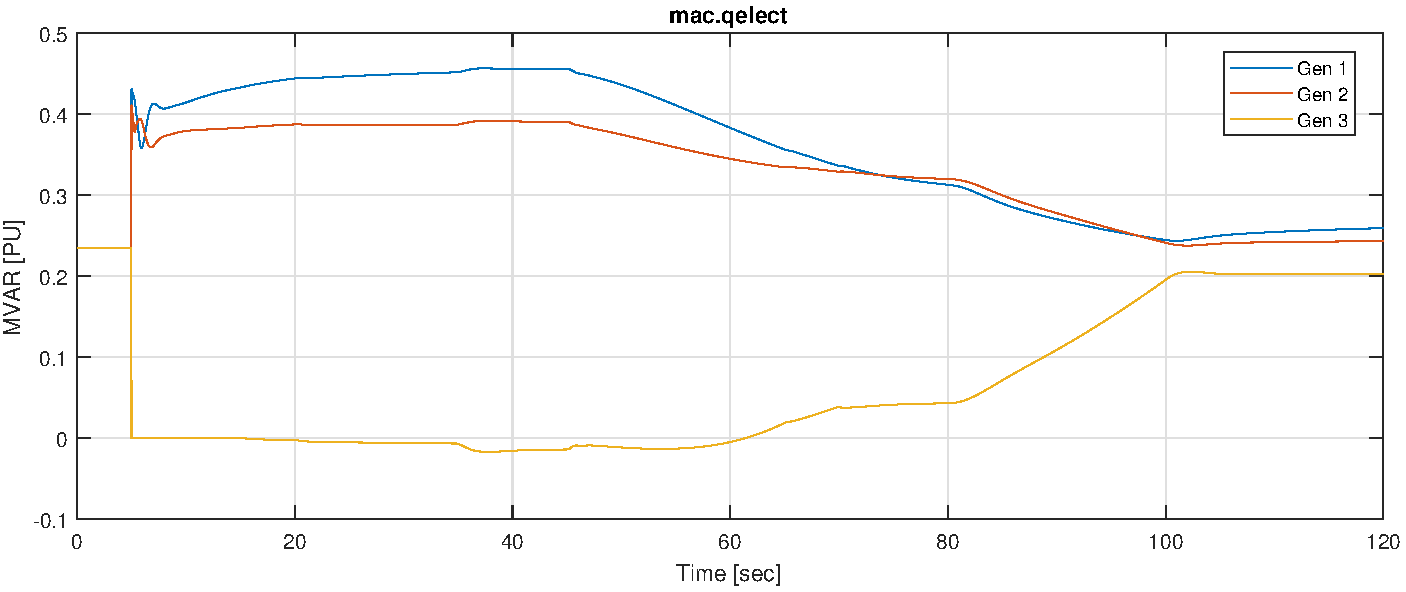
\includegraphics[width=\linewidth]{distinctQelect}

\pagebreak
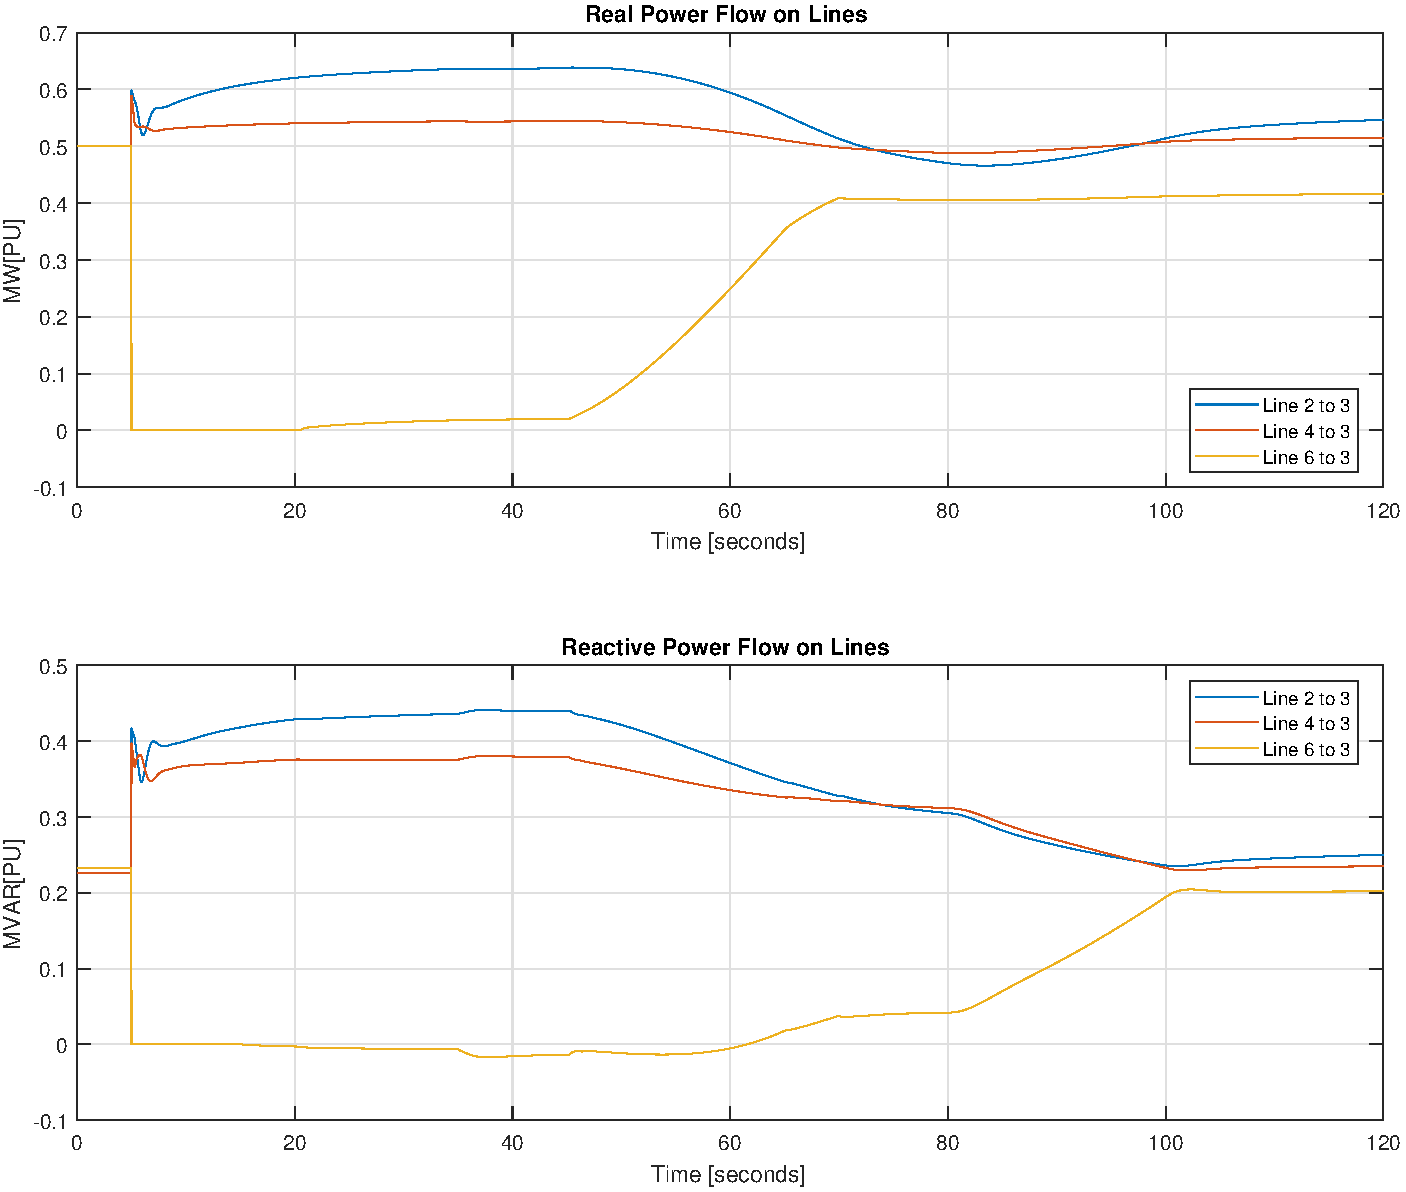
\includegraphics[width=\linewidth]{distinctLoadFlow}

\end{document}
